\documentclass[a4paper,12pt]{report}
\renewcommand\thechapter{\Roman{chapter}}
\usepackage[utf8]{inputenc}
\usepackage{lipsum}
\usepackage{kantlipsum}
\usepackage[calcwidth]{titlesec}
\usepackage{fix-cm} 
\usepackage[Sonny]{fncychap}
\usepackage{setspace}
\usepackage[natbibapa]{apacite}
\usepackage{pdflscape}
\usepackage{float}
\doublespacing
\setlength{\parindent}{0pt}
\renewcommand{\baselinestretch}{1.3} 

\titleformat{\chapter}[display]{\Large}{\centering
  \MakeUppercase{\chaptername}\quad{\Huge\thechapter}}{10pt}{\titlerule[.5pt]\vspace{10pt}\centering
  \MakeUppercase}[\vspace{10pt}{\titlerule[.5pt]}]% <-- spacing of title bar
\titlespacing{\chapter}{0pt}{-80pt}{1cm}% <-- spacing of title bar



\usepackage{amsthm, amsmath, amssymb, mathtools, mathbbol}
\numberwithin{equation}{section}
\theoremstyle{definition}
\newtheorem{thm}{Theorem}[section]
\newtheorem{Def}[thm]{Definition}
\newtheorem{prob}[thm]{Problem}
\newtheorem{rem}[thm]{Remark}

\usepackage{natbib}
\usepackage{graphicx}

\graphicspath{{graphics/}}

\begin{document}



\begin{center}


\Large NATIONAL UNIVERSITY OF SINGAPORE\\ 
\Large Master's of Computing (General-Track) \\ [0.2in]

\includegraphics[width=10cm]{1.nus_logo_full-horizontal} \\
\Large {\bf Alpha Tree Search and Machine Learning Approaches to Optimising Real Estate Portfolios}\\ [0.2in]
Leong Wei Ming \\
Supervisor: Professor Liu Li Li \\
Examiner: Professor Chin Wei Ngan \\ [0.3in]
Department of Computer Science \\
Internal Capstone Project for AY2023/2024
\end{center}


\chapter*{Abstract}
An internal project about applying genetic algorithm to search for optimal alphas.    
State the major contribution:

\chapter*{Declaration}
\begin{center}{\large
I hereby declare that this project report is my original work and it has been written by me in its entirety. I have duly acknowledged all the sources of information which have been used in this report. \\[0.5in]
This report has also not been submitted for any degree in any university previously.
}

\chapter*{Acknowledgement}
{\large
I would like to thank Professor Liu Lili for her guidance, support and encouragement throughout the course of this project. Working with Professor Lili has been a great learning experience, getting to learn much more about machine learning and its applications to finance in solving some challenges faced by industry practitioners. \\[0.5in]
Also many thanks to Professor Chin Wei Ngan for taking the time out to assess this project.

}
\end{center}
\setcounter{secnumdepth}{3}
\setcounter{tocdepth}{3}

\tableofcontents


\setcounter{chapter}{1}
\renewcommand{\thechapter}{\arabic{chapter}}
\pagenumbering{arabic}
\setcounter{chapter}{0}
\chapter{Introduction}
The saying goes that once a profitable trading formula has been discovered and traded on by enough people, its profits will be eroded away and it will cease to be profitable. Traders and investors appear to be playing a never-ending game of "Hide-and-Seek" in search of profitable trading strategies. Due to the evolving nature of the financial markets, traditional financial time-series forecasting models which are static in nature are becoming less effective than Machine Learning models and dynamic algorithms in identifying the best investments \citep{sheth_predicting_2023}. The success of Machine Learning has led to numerous research papers applying a myriad of Machine Learning techniques to predict stock prices \citep{obthong_survey_2020}. However, fewer papers apply these approaches in the Real Estate sector and these papers largely focus on future stock price prediction rather than portfolio allocation as a whole \citep{habbab_-depth_2024}. Many of these papers also use price-volume data without fundamental financial data as inputs. In 2022, the global real estate sector was worth more than \$380 trillion and worth more than the global equity and bond markets combined \citep{tostevin_total_2023}, with approximately 893 listed Real Estate Investment Trusts (REITs) \citep{nareit_global_2024}. Hence, addressing the research gaps in this sector is particularly valuable.



\section{Problem Definition}
The aim of this report is to develop an effective real estate portfolio optimisation model that maximises profits, minimises risks and outperforms the market indexes with a sharpe ratio of more than 2. A novel approach of applying Genetic Algorithms to search for outperforming Alpha formulas, as well as, three Machine Learning models, namely, Multiple Linear Regression (MLR), Neural Networks (NN) and Long-Short Term Memory (LSTM) are used to construct models. A trading agent is also constructed to allocate funds to the portfolio based on the results from the models. The input data to the Machine Learning models will be extended beyond price-volume data to include fundamental stock data. The models will be trained on 10 years worth of real market data. Then, the performances of these approaches will be compared with traditional financial models and the market indexes.


\section{Motivations}
Interviews of traders and financial journalists have revealed that both technical and fundamental analysis are used for forecasting investments, for shorter and medium to long term investment horizons respectively \citep{oberlechner_importance_2001}. Given that most investments in real estate are meant for the medium to long term, the lack of fundamental data inputs for REITs stock price predictions reveals a pressing need for fundamental data to be incorporated. \\ 


In the field of quantitative trading, quant firms seek to develop predictive algorithms for quantitative trading called "Alphas" that determine how capital is allocated to portfolios profitably \citep{tulchinsky_finding_2020}. What began with investment experts manually constructing Alpha formulas has gradually been replaced with automated alpha mining techniques that employ Machine Learning algorithms \citep{wang_alpha-gpt_2023}. There appears to be an opportunity to apply the concept of quantitative finance Alphas for Real Estate portfolio allocation. In addition, researchers have been inspired by Charles Darwin's theory of evolution \citep{ruse_charles_1975} to develop a Genetic Algorithm and have applied it in finance \citep{aguilar-rivera_genetic_2015}. Synthesising these two ideas, presents a new and innovative approach to use Genetic Algorithms to search for Alphas in the Real Estate sector. \\

Lastly, as most of past research is centered on price prediction, there is a need to develop trade execution logic to allocate portfolios based on these predictions.




\section{Major Contributions and Creativity}
The first major contribution of this project is the analysis on REITs stock datasets with more than 150 features of technical and fundamental indicators. This expands the dimensionality of the input training data significantly beyond price-volume features to incorporate REIT company data from financial statements. The comprehensive dataset covers 150 out of the total worldwide population of 893 REITs and includes up to 20 years of historical data.\\

Creativity is demonstrated in the writing of a Genetic Search Algorithm that searches for outperforming REIT Alphas. It resulted in the second contribution of a trading model with superior returns that significantly outperforms the market indexes.\\ 

The third contribution is the implementation of a trading agent or trade execution logic that acts on individual REIT price predictions to allocate funds to selected REITS in a portfolio.\\

Overall, this research paper has expanded the body of knowledge on the application of Alphas and Machine Learning models in Optimising Real Estate Portfolios.


\titleformat{\chapter}[block]
  {\normalfont\huge\bfseries}{\thechapter.}{1em}{\Huge\centering}
\titlespacing*{\chapter}{0pt}{150pt}{0pt}
\setcounter{chapter}{0}
\renewcommand{\thechapter}{\Roman{chapter}}
\chapter{Background}



\titleformat{\chapter}[display]{\Large}{\centering
  \MakeUppercase{\chaptername}\quad{\Huge\thechapter}}{10pt}{\titlerule[.5pt]\vspace{10pt}\centering
  \MakeUppercase}[\vspace{10pt}{\titlerule[.5pt]}]% <-- spacing of title bar
\titlespacing{\chapter}{0pt}{-23pt}{1cm}% <-- spacing of title bar
\renewcommand{\thechapter}{\arabic{chapter}}
\pagenumbering{arabic}
\chapter{Financial Terminology and Concepts}
\section{Key Terms}
\subsection{Stock}
\subsection{Real Estate Investment Trusts (REITs)}
\subsection{Portfolio}

\section{Evaluating Investments with Data}
\subsection{Technical Analysis with Price Volume Data}
\subsubsection{Profits and Loss (PnL)}
\subsubsection{Risk and Volatility}
\subsubsection{Sharpe Ratio}
\subsection{Fundamental Analysis with Financial Statements}
\subsubsection{Income Statement}
\subsubsection{Balance Sheet}
\subsubsection{Cash Flow Statement}
\subsection{Alpha Formulas}
\subsection{Other Methods of Analyses}

\chapter{Literature Review of Portfolio Optimisation Techniques}
\section{Optimal Portfolio Theory}
\section{Traditional Time-Series Analysis}
\section{Machine Learning Techniques}
\section{Comparison of Techniques}
\subsection{Scope}
\subsection{Profitability}
\subsection{Predictive Accuracy}

\titleformat{\chapter}[block]
  {\normalfont\huge\bfseries}{\thechapter.}{1em}{\Huge\centering}
\titlespacing*{\chapter}{0pt}{150pt}{0pt}
\setcounter{chapter}{1}
\renewcommand{\thechapter}{\Roman{chapter}}
\chapter{Innovation}


\titleformat{\chapter}[display]{\Large}{\centering
  \MakeUppercase{\chaptername}\quad{\Huge\thechapter}}{0pt}{\titlerule[.5pt]\vspace{10pt}\centering
  \MakeUppercase}[\vspace{10pt}{\titlerule[.5pt]}]% <-- spacing of title bar
\titlespacing{\chapter}{0pt}{-80pt}{1cm}% <-- spacing of title bar
\renewcommand{\thechapter}{\arabic{chapter}}
\setcounter{chapter}{3}
\pagenumbering{arabic}
\chapter{Datasets}
\section{Extended Fundamental Data Features}
\section{Feature Selection with Decision Trees}

\def\fillandplacepagenumber{%
 \par\pagestyle{empty}%
 \vbox to 0pt{\vss}\vfill
 \vbox to 0pt{\baselineskip0pt
   \hbox to\linewidth{\hss}%
   \baselineskip\footskip
   \hbox to\linewidth{%
     \hfil\thepage\hfil}\vss}}



\chapter{Methodology}

\begin{figure}[H]
\centerline{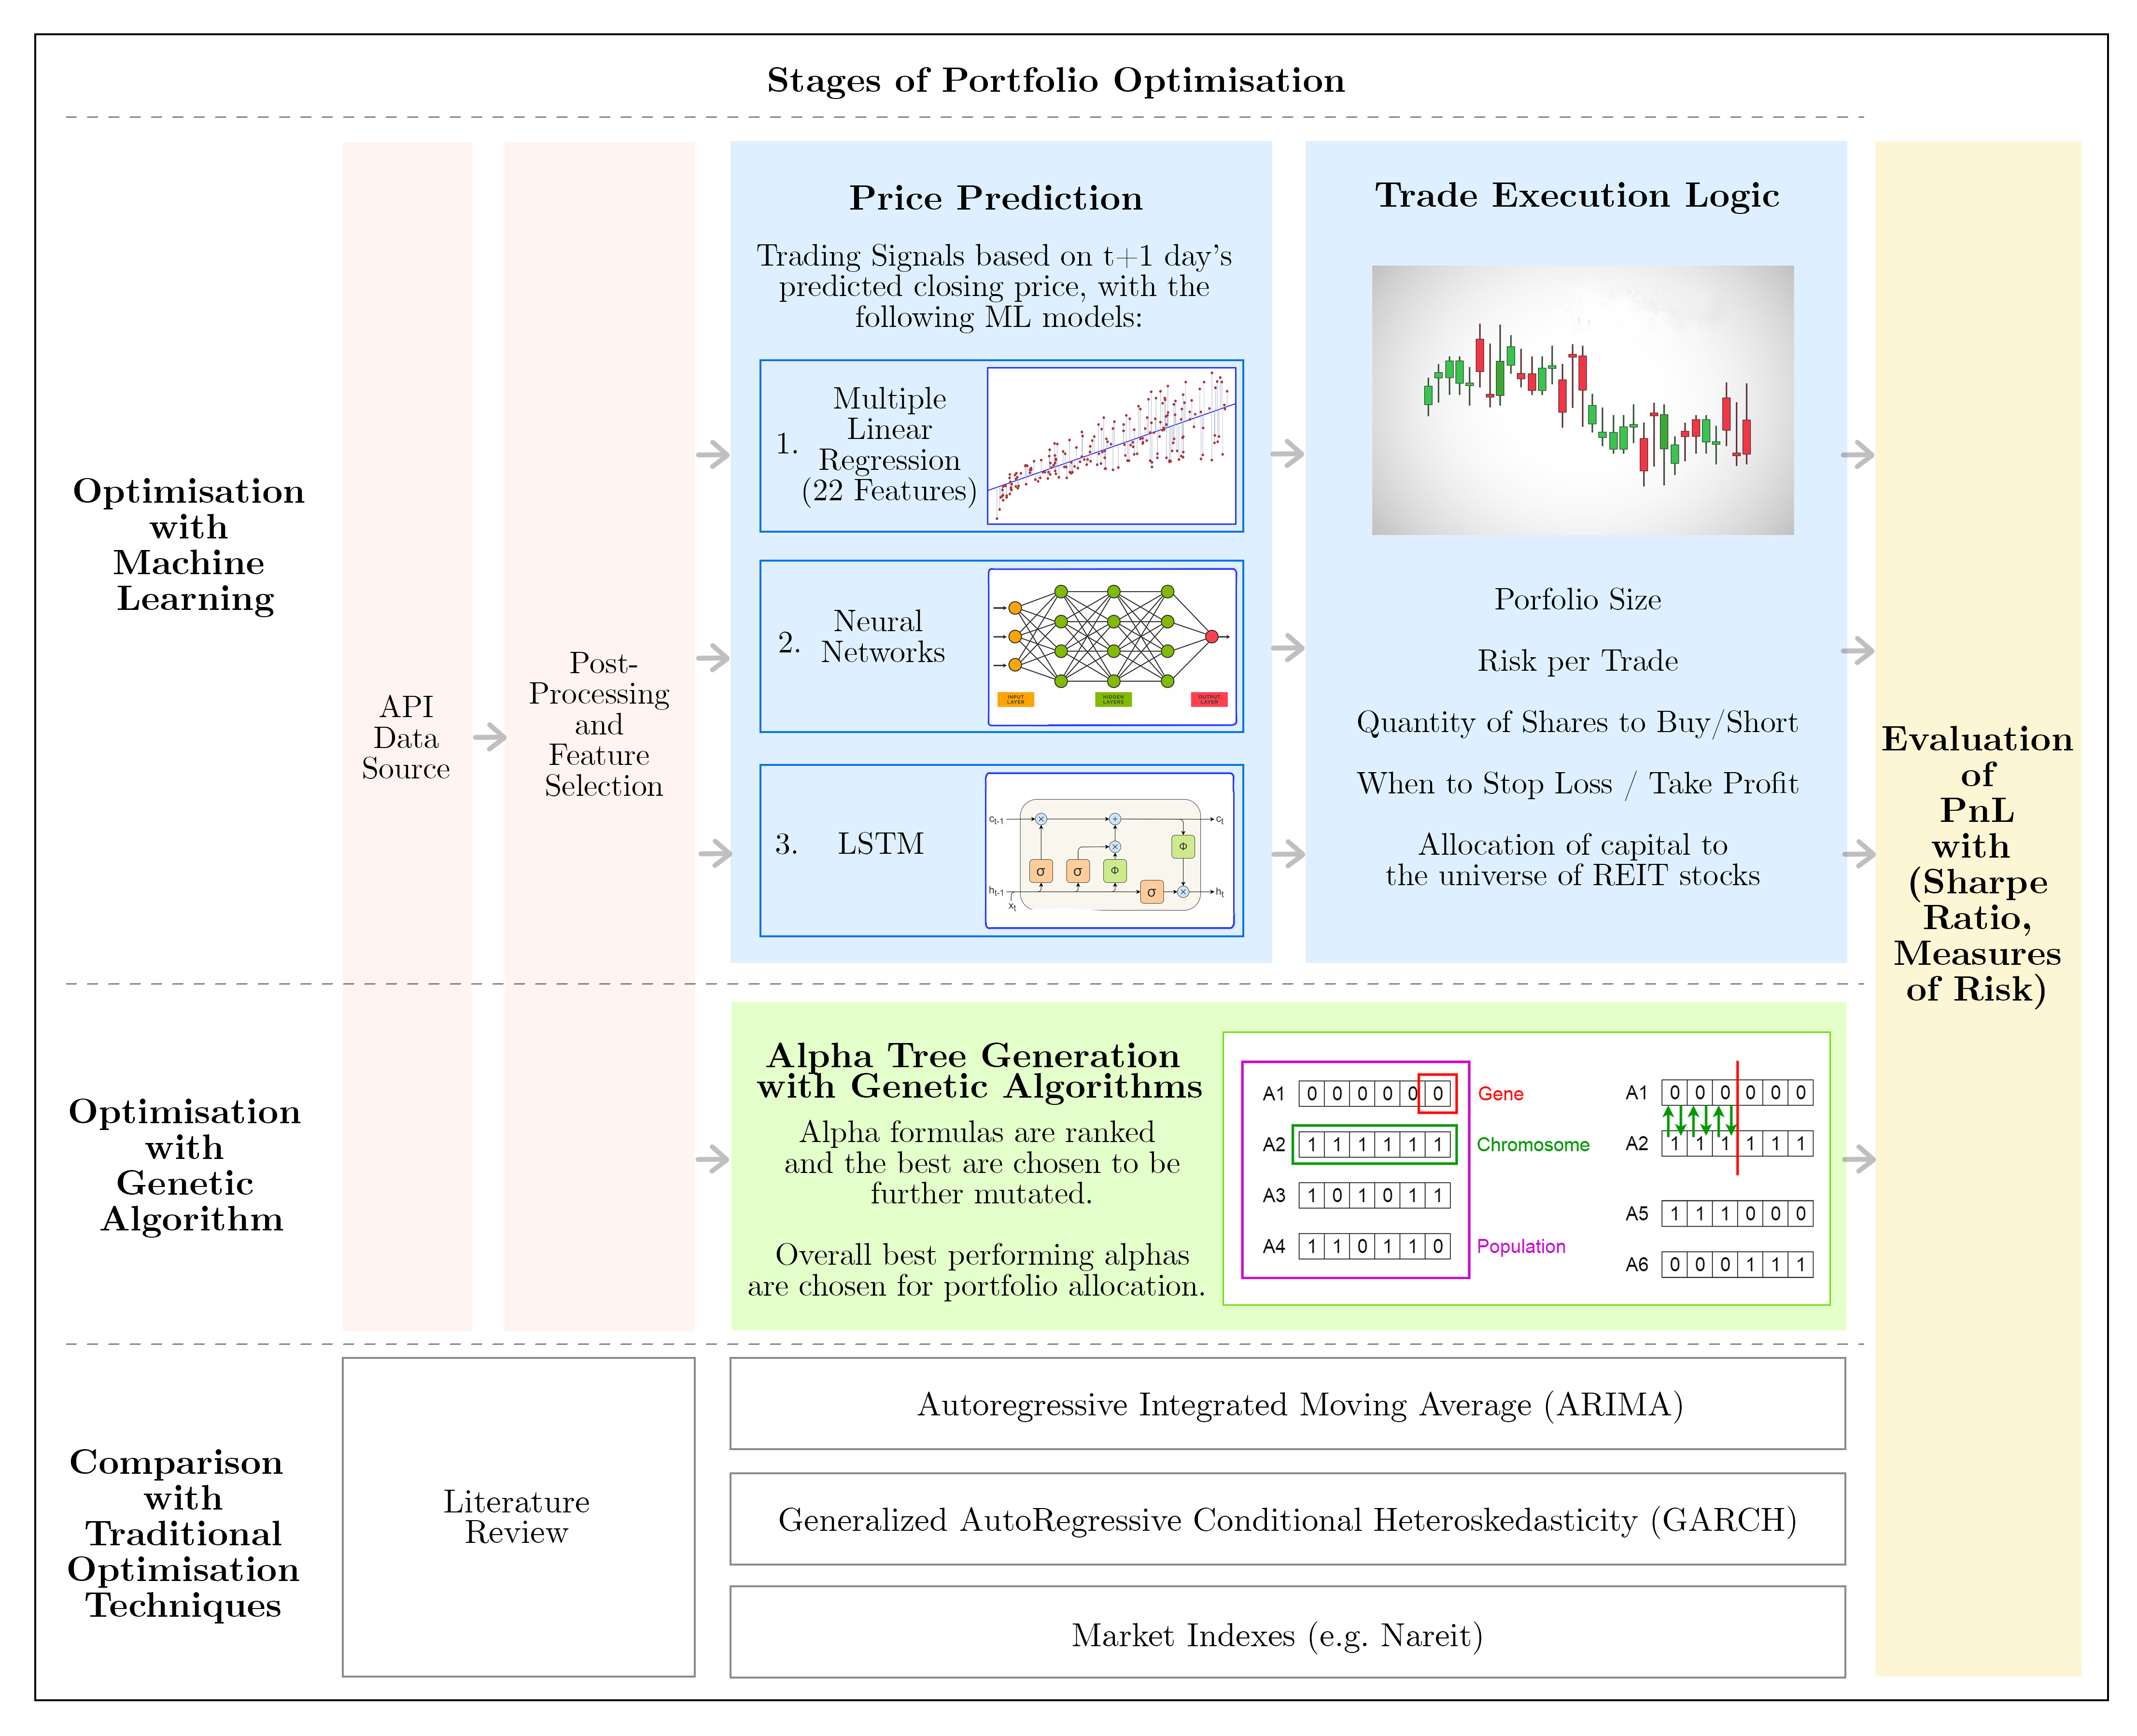
\includegraphics[width=21cm]{Overall_Methodology}}
\caption{Write some caption here}\label{visina8}
\end{figure}



%\begin{landscape}
%\fillandplacepagenumber
%\end{landscape}


\section{Machine Learning for REITs Portfolio Optimisation}
\subsection{MLR / NN / LSTM Predictions with Extended Features}
\subsection{Trade Execution Logic}
\subsection{Performance Evaluation}
\section{Genetic Algorithm Search for Outperforming Alphas}
\subsection{Alpha Tree}
\subsection{Application of Genetic Algorithms to Alpha Trees}
\subsubsection{Objective Function}
\subsubsection{Selection}
\subsubsection{Crossover}
\subsubsection{Mutation}
\subsection{Portfolio Allocation Using Alpha}
\subsection{Performance Evaluation}


\titleformat{\chapter}[block]
  {\normalfont\huge\bfseries}{\thechapter.}{1em}{\Huge\centering}
\titlespacing*{\chapter}{0pt}{150pt}{0pt}
\setcounter{chapter}{2}
\renewcommand{\thechapter}{\Roman{chapter}}
\chapter{Experiments}

\titleformat{\chapter}[display]{\Large}{\centering
  \MakeUppercase{\chaptername}\quad{\Huge\thechapter}}{10pt}{\titlerule[.5pt]\vspace{10pt}\centering
  \MakeUppercase}[\vspace{10pt}{\titlerule[.5pt]}]% <-- spacing of title bar
\titlespacing{\chapter}{0pt}{-23pt}{1cm}% <-- spacing of title bar
\renewcommand{\thechapter}{\arabic{chapter}}
\setcounter{chapter}{5}
\pagenumbering{arabic}
\chapter{Post-processed Financial Datasets}

\chapter{Machine Learning Results}
\section{Evaluating Stock Price Predictions}
\subsection{Multiple Linear Regression (MLR)}
\subsection{Neural Networks (NN)}
\subsection{Long-Short Term Memory (LSTM)}
\section{Trade Execution Results with Different Parameters}
\section{Overall Evaluation of Performances}


\chapter{Alpha Tree Search Results}
\section{Alphas Generated}
\subsection{Initial Set}
\subsection{Intermediate Alphas}
\subsection{Best Performing Alphas}
\section{Portfolio Allocation Results with Best Performing Alphas}
\section{Overall Evaluation of Performance}



\chapter{Conclusion}
\section{Benchmarking Against Index Funds}
\section{Comparing Results with Literature Review}
\section{Key Findings}
\section{Major Contribution and Creativity}
\section{Future Work}
\subsection{More Operators and Features for Alphas}


\begin{figure}[h!]
\centering
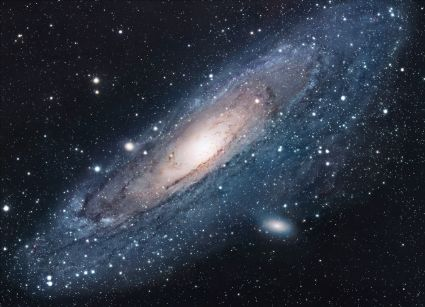
\includegraphics[scale=1.7]{universe}
\caption{The Universe}
\label{fig:universe}
\end{figure}



\bibliographystyle{apacite}
\bibliography{references}
\end{document}
